%=== Materials and Methods ===
\chapter{2. Facade Pattern}
\section{Đặt vấn đề - Rạp hát tại gia}
 Trước khi chúng ta đi chi tiết vào Facade Pattern, hãy tưởng tượng việc xây dựng rạp hát cho ngôi nhà thân yêu của mình\\[0.15in]
 Sau dày công nghiên cứu, cuối cùng ta có được một hệ thống hoàn chỉnh với một đĩa DVD, máy chiếu kỹ thuật số, màn hình tự động và cả một chút bỏng ngô nữa:

%Adding a figure
\begin{figure}[!htb]
    \centering
    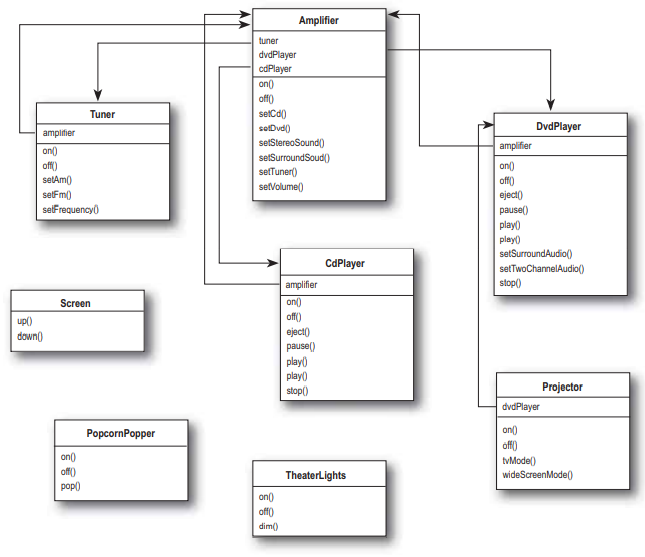
\includegraphics[width=\textwidth]{fig/Facade/TheaterSystem.png}/
\end{figure}
\newpage
Lấy 1 chiếc đĩa DVD, pha tách trà và thư giãn. Nhưng mà chờ đã, trước khi xem phim ta cần phải thực hiện những việc sau: bật bắp rang bơ lên, giảm độ sáng, đặt màn hình xuống, bật máy chiếu lên,....  Với việc gọi lớp và phương thức thông thường

\begin{figure}[!htb]
    \centering
    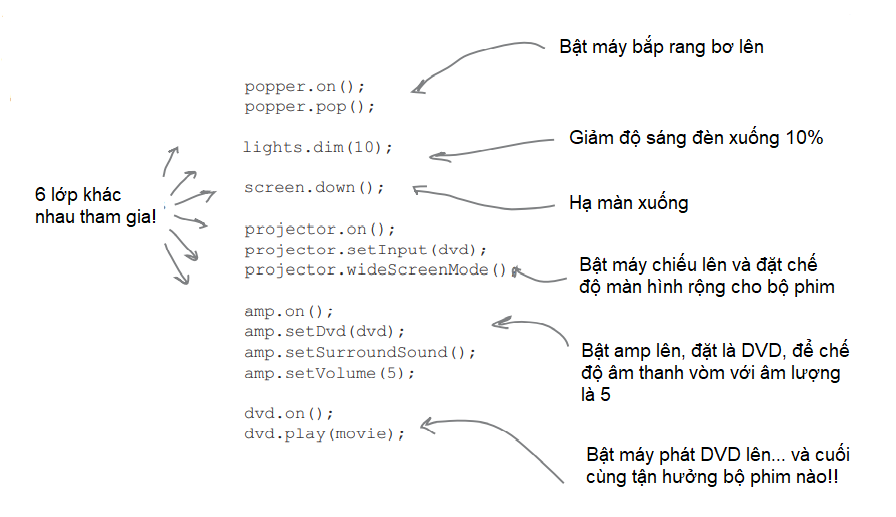
\includegraphics[width=\textwidth]{fig/Facade/TheaterWithClassMethodCalling.png}/
\end{figure}
\textbf{Việc này phát sinh 1 số vấn đề như sau:}\smallskip

- Khi bộ phim kết thúc, làm sao để tắt mọi thứ? Hay phải làm hết những việc này theo chiều ngược lại?\smallskip

- Việc nghe đĩa CD hay Radio cũng phức tạp không kém gì DVD?\smallskip

- Khi nâng cấp hệ thống, chương trình trong Client cũng phải sửa đi\bigskip

\textbf{Facade Pattern} là giải pháp cho những vấn đề trên. Mục đích chính là để giảm độ phức tạp trong hệ thống và đơn giản hóa interface. Không những vậy, Facade thể hiện tính trừu tượng: giấu đi những thứ được triển khai bên trong và chỉ để lại Interface cho Client dễ dàng sử dụng
\newpage
\section{Định nghĩa và Mô hình cấu trúc}
\subsection{Định nghĩa}

\textbf{Facade Pattern} cung cấp một giao diện thống nhất một tập hợp những giao diện trong một hệ thống con. Facade xác định một giao diện ở mức cao để thuận tiện trong việc sử dụng hệ thống con

\subsection{Mô hình cấu trúc}

Mô hình cấu trúc của Facade Pattern được biểu diễn như sau:
\begin{figure}[!htb]
    \centering
    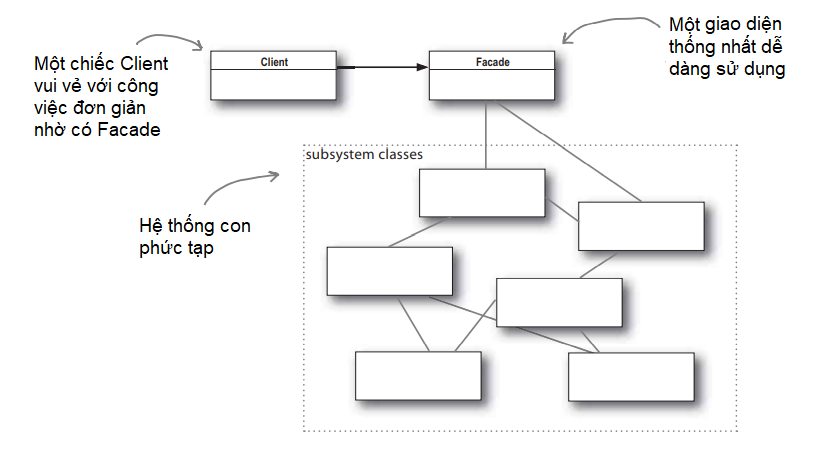
\includegraphics[width=\textwidth]{fig/Facade/FacadeDiagram.png}/
\end{figure}
\newpage
\section{Facade Pattern: Rạp hát - Set ON!}

Nhờ vào mô hình cấu trúc đã được định nghĩa ở trên, ta có thể nâng cấp rạp hát với mô hình như sau:
\begin{figure}[!htb]
    \centering
    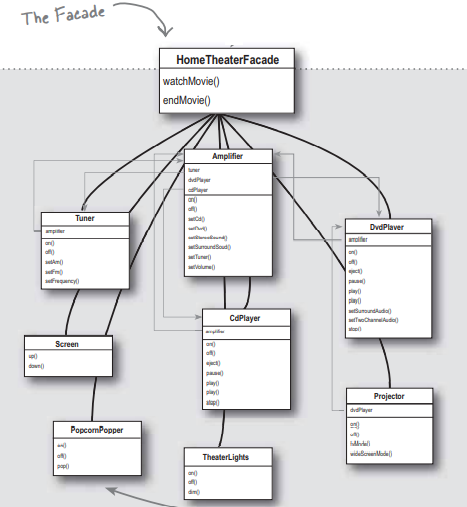
\includegraphics[width=\textwidth]{fig/Facade/TheaterFacade.png}/
\end{figure}

Về mặt ý tưởng, ta sẽ tạo một lớp mới tên là \textbf{HomeTheaterFacade}, nơi chứa một vài phương thức như \textbf{watchMovie()}. Lúc này, lớp Facade sẽ coi những thành phần trong rạp như một hệ thống con và gọi chúng trong phương thức \textbf{watchMovie()}. Client sẽ gọi những phương thức trong lớp Facade, không phải hệ thống con. Nói cách khác, khi cần xem phim thì việc gọi phương thức \textbf{watchMovie()} và phương thức đó sẽ tự động kết nối đến đèn, đầu đĩa DVD, máy chiếu, bộ khuếch đại,...
\newpage
Dưới đây là doạn code minh họa cho lớp HomeTheaterFacade:
\begin{figure}[!htb]
    \centering
    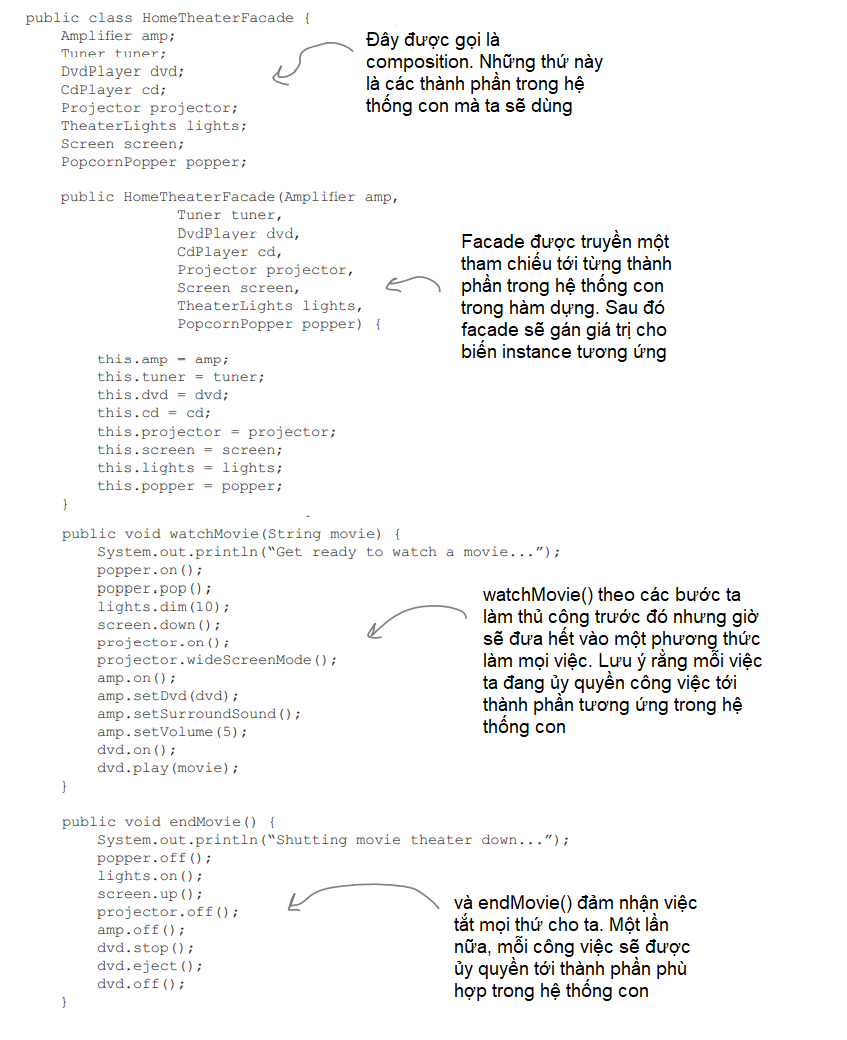
\includegraphics[width=\textwidth]{fig/Facade/HomeTheaterFacade.png}/
\end{figure}
\newpage

Đến giờ thưởng thức phim sau bao công sức:
\begin{figure}[!htb]
    \centering
    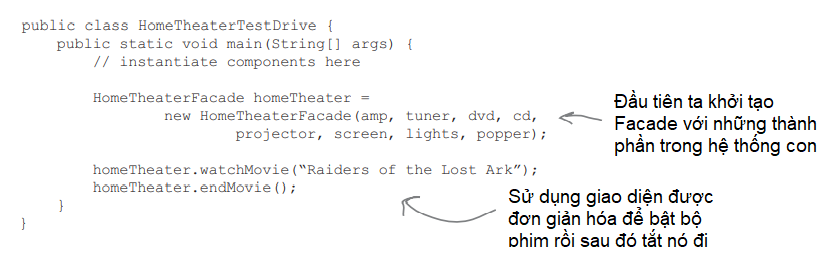
\includegraphics[width=\textwidth]{fig/Facade/TheaterMain.png}/
\end{figure}

\section{Thực tế}

Trong ET++ application framework [WGM88], một ứng dụng có thể được tích hợp sẵn các công cụ duyệt để kiểm tra các đối tượng của nó tại thời điểm chạy. Những công cụ duyệt này được triển khai trong một hệ thống con riêng biệt bao gồm một lớp \textbf{Facade} được gọi là "ProgrammingEnvironment". Những facade này định nghĩa các thao tác như InspectObject và InspectClass để truy cập các trình duyệt\\[0.1in]
Hệ điều hành The Choices [CIRM93] sử dụng facade để hợp thành nhiều framework thành một. Có những phần chính trong Choices là quy trình, không gian lưu trữ và không gian địa chỉ. Ứng với mỗi phần sẽ có một hệ thống con tương ứng, triển khai như một framework hỗ trợ chuyển Choices trên nhiều nền tảng phần cứng khác nhau. 2 trong những hệ thống con có một "representative" (i.e.facade). Những representatives là FileSystemlnterface (không gian lưu trữ) và Domain (không gian địa chỉ)

%=== END OF MM ===
\newpage
